\documentclass{article}
\usepackage[utf8]{inputenc}
\usepackage[T1]{fontenc}
\usepackage{amsmath}
\usepackage{tkz-tab}
\usepackage[framemethod=tikz]{mdframed}
\usepackage{xcolor}
\usepackage{pgfplots}
\pgfplotsset{compat=1.3}
\usetikzlibrary{positioning, fit, calc}
\tikzset{block/.style={draw, thick, text width=2cm ,minimum height=1.3cm, align=center},   
	line/.style={-latex}     
}
\tikzset{blocktext/.style={draw, thick, text width=5.2cm ,minimum height=1.3cm, align=center},   
	line/.style={-latex}     
}
\tikzset{font=\footnotesize}

\begin{document}

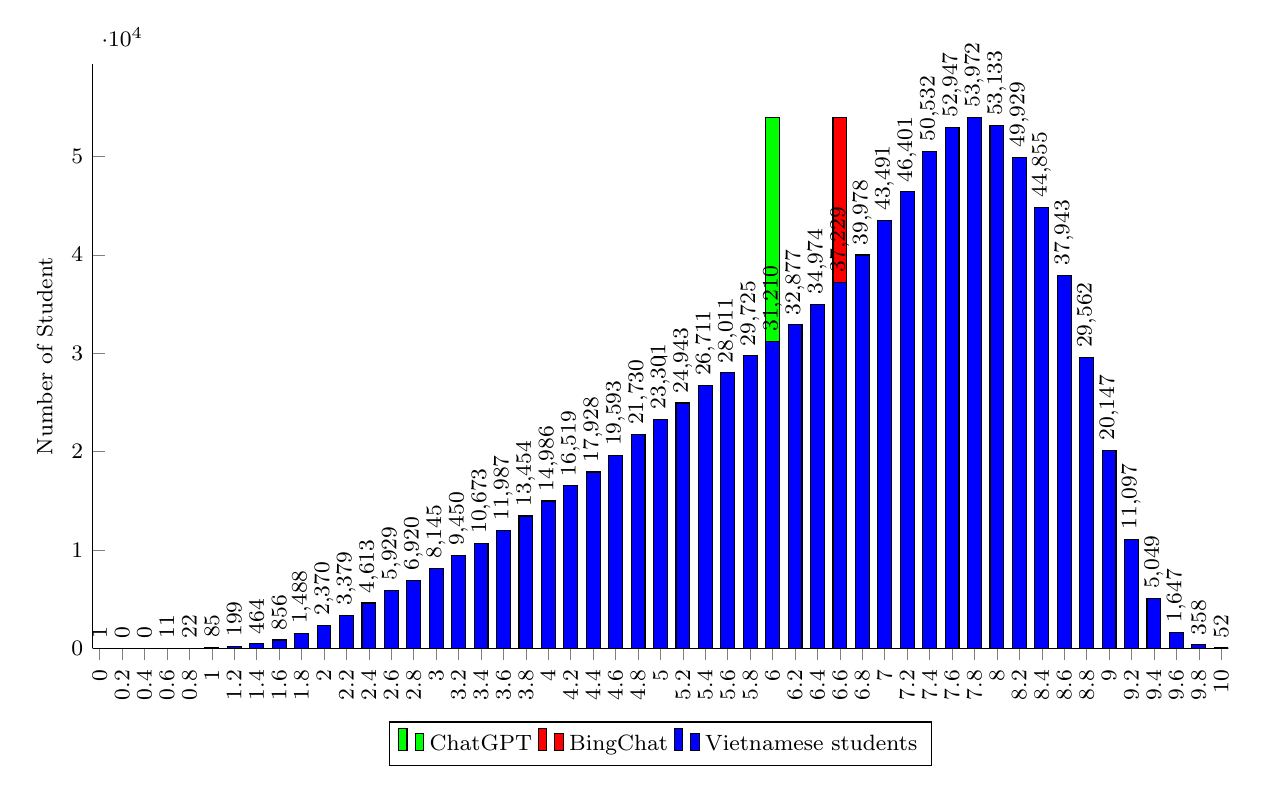
\begin{tikzpicture}
				\begin{axis}[
					legend style={at={(0.5,-0.125)}, 	
						anchor=north,legend columns=-1}, 
					symbolic x coords={
						0,
						0.2,
						0.4,
						0.6,
						0.8,
						1,
						1.2,
						1.4,
						1.6,
						1.8,
						2,
						2.2,
						2.4,
						2.6,
						2.8,
						3,
						3.2,
						3.4,
						3.6,
						3.8,
						4,
						4.2,
						4.4,
						4.6,
						4.8,
						5,
						5.2,
						5.4,
						5.6,
						5.8,
						6,
						6.2,
						6.4,
						6.6,
						6.8,
						7,
						7.2,
						7.4,
						7.6,
						7.8,
						8,
						8.2,
						8.4,
						8.6,
						8.8,
						9,
						9.2,
						9.4,
						9.6,
						9.8,
						10,
					},
					%xtick=data,
					hide axis,
					ybar,
					bar width=5pt,
					ymin=0,
					%enlarge x limits,
					%nodes near coords,   
					every node near coord/.append style={rotate=90, anchor=west},
					width=\textwidth, 
					enlarge x limits={abs=0.5*\pgfplotbarwidth},
					height=9cm, 
					width=16cm,
					axis x line*=bottom, axis y line*=left
					]
					\addplot [fill=green] coordinates {
						(0,0)
					};
					\addplot [fill=red] coordinates {
						(5,0)
					};	
					\addplot [fill=blue] coordinates {
						(10,0)
					};	
					\legend{ChatGPT, BingChat,Vietnamese students }	
				\end{axis}
				
				\begin{axis}[
					symbolic x coords={
						0,
						0.2,
						0.4,
						0.6,
						0.8,
						1,
						1.2,
						1.4,
						1.6,
						1.8,
						2,
						2.2,
						2.4,
						2.6,
						2.8,
						3,
						3.2,
						3.4,
						3.6,
						3.8,
						4,
						4.2,
						4.4,
						4.6,
						4.8,
						5,
						5.2,
						5.4,
						5.6,
						5.8,
						6,
						6.2,
						6.4,
						6.6,
						6.8,
						7,
						7.2,
						7.4,
						7.6,
						7.8,
						8,
						8.2,
						8.4,
						8.6,
						8.8,
						9,
						9.2,
						9.4,
						9.6,
						9.8,
						10,
					},
					%xtick=data,
					hide axis,
					x tick label style={rotate=90,anchor=east},
					ybar,
					bar width=5pt,
					ymin=0,
					%enlarge x limits,
					%nodes near coords,   
					every node near coord/.append style={rotate=90, anchor=west},
					width=\textwidth, 
					enlarge x limits={abs=0.5*\pgfplotbarwidth},
					height=9cm, 
					width=16cm,
					axis x line*=bottom, axis y line*=left
					]
					\addplot [fill=green] coordinates {
						(0,0)
						(0.2,0)
						(0.4,0)
						(0.6,0)
						(0.8,0)
						(1,0)
						(1.2,0)
						(1.4,0)
						(1.6,0)
						(1.8,0)
						(2,0)
						(2.2,0)
						(2.4,0)
						(2.6,0)
						(2.8,0)
						(3,0)
						(3.2,0)
						(3.4,0)
						(3.6,0)
						(3.8,0)
						(4,0)
						(4.2,0)
						(4.4,0)
						(4.6,0)
						(4.8,0)
						(5,0)
						(5.2,0)
						(5.4,0)
						(5.6,0)
						(5.8,0)
						(6,55000)
						(6.2,0)
						(6.4,0)
						(6.6,0)
						(6.8,0)
						(7,0)
						(7.2,0)
						(7.4,0)
						(7.6,0)
						(7.8,0)
						(8,0)
						(8.2,0)
						(8.4,0)
						(8.6,0)
						(8.8,0)
						(9,0)
						(9.2,0)
						(9.4,0)
						(9.6,0)
						(9.8,0)
						(10,0)
						
					};	
				\end{axis}
				
				\begin{axis}[ 
					symbolic x coords={
						0,
						0.2,
						0.4,
						0.6,
						0.8,
						1,
						1.2,
						1.4,
						1.6,
						1.8,
						2,
						2.2,
						2.4,
						2.6,
						2.8,
						3,
						3.2,
						3.4,
						3.6,
						3.8,
						4,
						4.2,
						4.4,
						4.6,
						4.8,
						5,
						5.2,
						5.4,
						5.6,
						5.8,
						6,
						6.2,
						6.4,
						6.6,
						6.8,
						7,
						7.2,
						7.4,
						7.6,
						7.8,
						8,
						8.2,
						8.4,
						8.6,
						8.8,
						9,
						9.2,
						9.4,
						9.6,
						9.8,
						10,
					},
					%xtick=data,
					hide axis,
					ybar,
					bar width=5pt,
					ymin=0,
					%enlarge x limits,
					%nodes near coords,   
					every node near coord/.append style={rotate=90, anchor=west},
					width=\textwidth, 
					enlarge x limits={abs=0.5*\pgfplotbarwidth},
					height=9cm, 
					width=16cm,
					axis x line*=bottom, axis y line*=left
					]
					\addplot [fill=red] coordinates {
						(0,0)
						(0.2,0)
						(0.4,0)
						(0.6,0)
						(0.8,0)
						(1,0)
						(1.2,0)
						(1.4,0)
						(1.6,0)
						(1.8,0)
						(2,0)
						(2.2,0)
						(2.4,0)
						(2.6,0)
						(2.8,0)
						(3,0)
						(3.2,0)
						(3.4,0)
						(3.6,0)
						(3.8,0)
						(4,0)
						(4.2,0)
						(4.4,0)
						(4.6,0)
						(4.8,0)
						(5,0)
						(5.2,0)
						(5.4,0)
						(5.6,0)
						(5.8,0)
						(6,0)
						(6.2,0)
						(6.4,0)
						(6.6,55000)
						(6.8,0)
						(7,0)
						(7.2,0)
						(7.4,0)
						(7.6,0)
						(7.8,0)
						(8,0)
						(8.2,0)
						(8.4,0)
						(8.6,0)
						(8.8,0)
						(9,0)
						(9.2,0)
						(9.4,0)
						(9.6,0)
						(9.8,0)
						(10,0)
					};	
				\end{axis}			
				\begin{axis}[
					ylabel={Number of Student},
					symbolic x coords={
						0,
						0.2,
						0.4,
						0.6,
						0.8,
						1,
						1.2,
						1.4,
						1.6,
						1.8,
						2,
						2.2,
						2.4,
						2.6,
						2.8,
						3,
						3.2,
						3.4,
						3.6,
						3.8,
						4,
						4.2,
						4.4,
						4.6,
						4.8,
						5,
						5.2,
						5.4,
						5.6,
						5.8,
						6,
						6.2,
						6.4,
						6.6,
						6.8,
						7,
						7.2,
						7.4,
						7.6,
						7.8,
						8,
						8.2,
						8.4,
						8.6,
						8.8,
						9,
						9.2,
						9.4,
						9.6,
						9.8,
						10,
					},
					xtick=data,
					x tick label style={rotate=90,anchor=east},
					ybar,
					bar width=5pt,
					ymin=0,
					%enlarge x limits,
					nodes near coords,   
					every node near coord/.append style={rotate=90, anchor=west},
					width=\textwidth, 
					enlarge x limits={abs=0.5*\pgfplotbarwidth},
					height=9cm, 
					width=16cm,
					axis x line*=bottom, axis y line*=left
					]
					\addplot [fill=blue] coordinates {
						(0,1)
						(0.2,0)
						(0.4,0)
						(0.6,11)
						(0.8,22)
						(1,85)
						(1.2,199)
						(1.4,464)
						(1.6,856)
						(1.8,1488)
						(2,2370)
						(2.2,3379)
						(2.4,4613)
						(2.6,5929)
						(2.8,6920)
						(3,8145)
						(3.2,9450)
						(3.4,10673)
						(3.6,11987)
						(3.8,13454)
						(4,14986)
						(4.2,16519)
						(4.4,17928)
						(4.6,19593)
						(4.8,21730)
						(5,23301)
						(5.2,24943)
						(5.4,26711)
						(5.6,28011)
						(5.8,29725)
						(6,31210)
						(6.2,32877)
						(6.4,34974)
						(6.6,37229)
						(6.8,39978)
						(7,43491)
						(7.2,46401)
						(7.4,50532)
						(7.6,52947)
						(7.8,53972)
						(8,53133)
						(8.2,49929)
						(8.4,44855)
						(8.6,37943)
						(8.8,29562)
						(9,20147)
						(9.2,11097)
						(9.4,5049)
						(9.6,1647)
						(9.8,358)
						(10,52)		
					};	
					
				\end{axis}
			\end{tikzpicture}

\end{document}